\hypertarget{pf__daemon_8c}{
\section{pf\_\-daemon.c File Reference}
\label{pf__daemon_8c}\index{pf\_\-daemon.c@{pf\_\-daemon.c}}
}
{\tt \#include $<$stdio.h$>$}\par
{\tt \#include $<$stdlib.h$>$}\par
{\tt \#include $<$unistd.h$>$}\par
{\tt \#include $<$errno.h$>$}\par
{\tt \#include $<$stdbool.h$>$}\par
{\tt \#include $<$dbus/dbus.h$>$}\par
{\tt \#include \char`\"{}libphonefirewall.h\char`\"{}}\par


Include dependency graph for pf\_\-daemon.c:\nopagebreak
\begin{figure}[H]
\begin{center}
\leavevmode
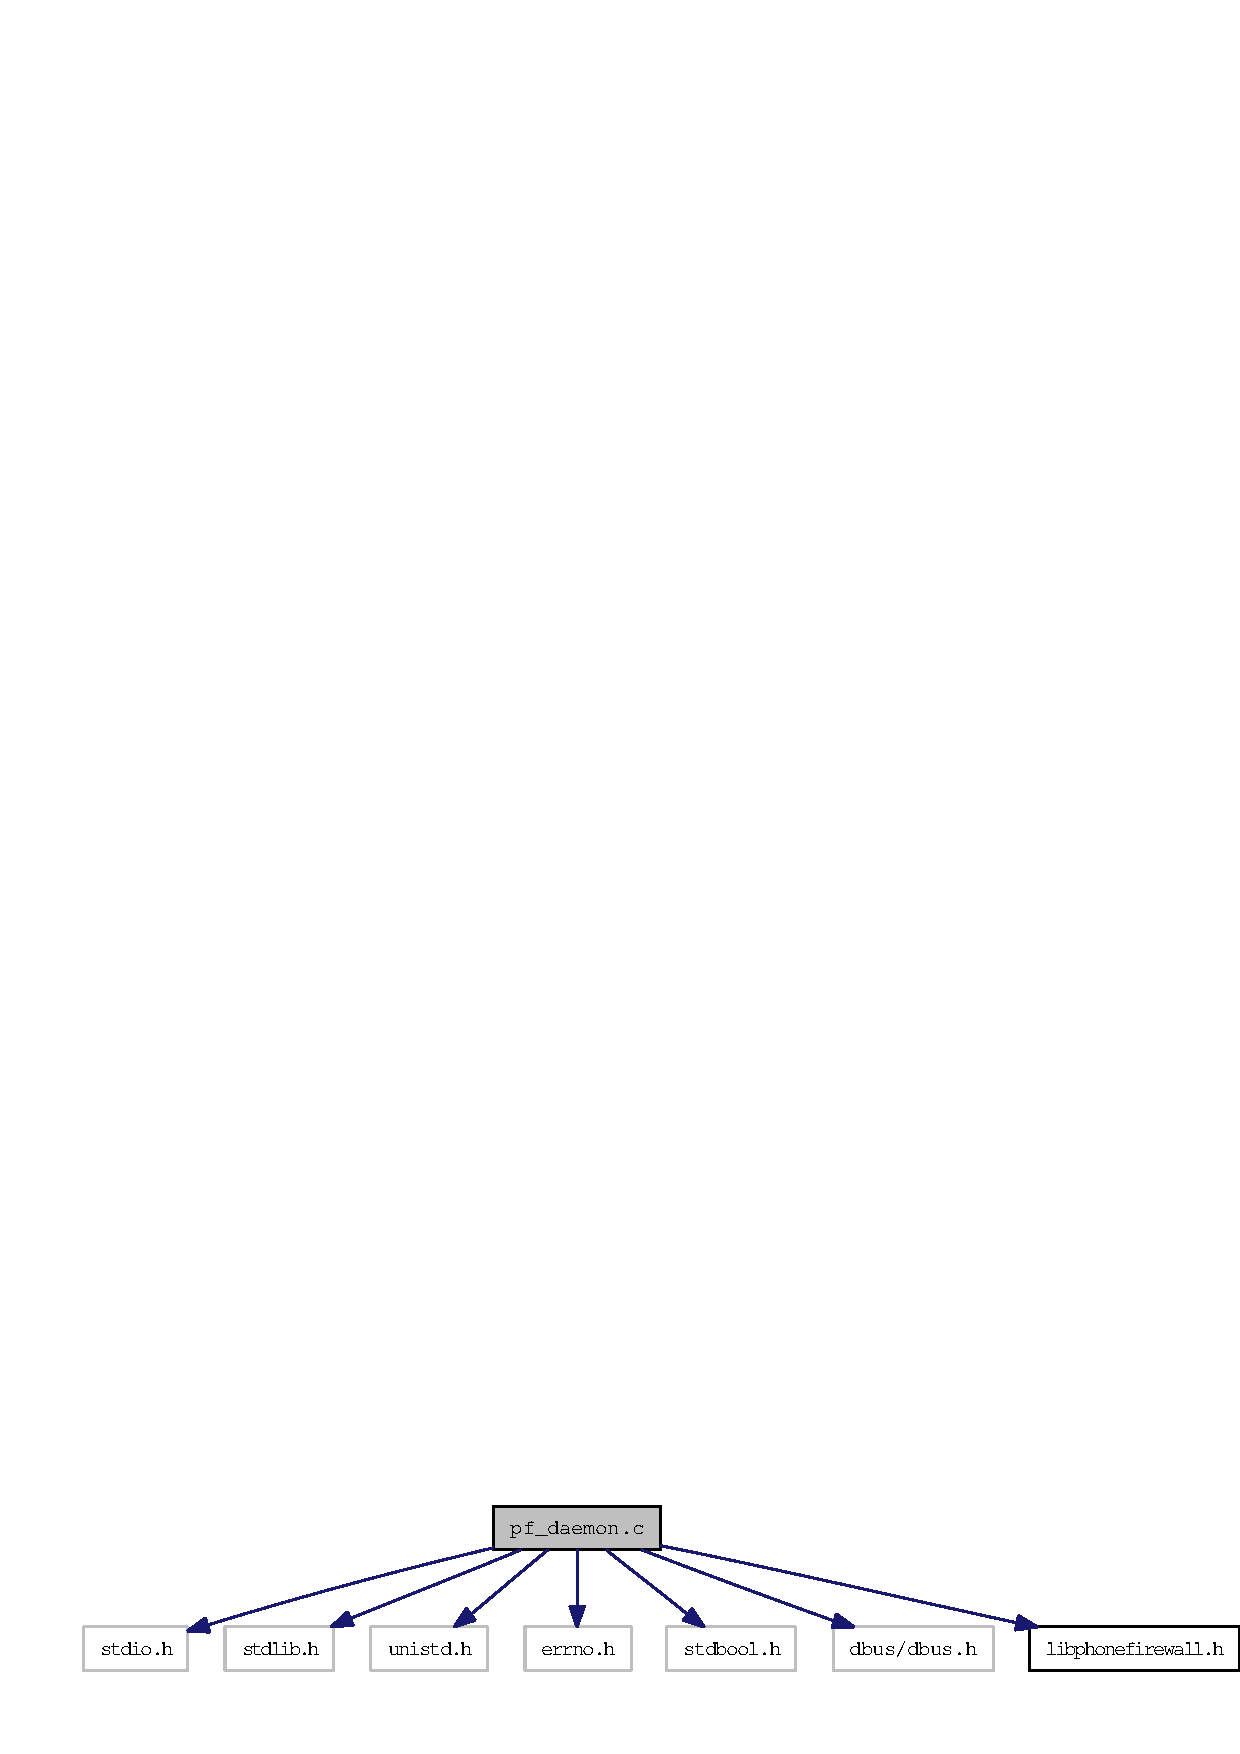
\includegraphics[width=299pt]{pf__daemon_8c__incl}
\end{center}
\end{figure}
\subsection*{Defines}
\begin{CompactItemize}
\item 
\#define \hyperlink{pf__daemon_8c_551ae9e7796a78ff54bc98eef4e74498}{LOCKFILE}~\char`\"{}.lock\char`\"{}
\end{CompactItemize}
\subsection*{Functions}
\begin{CompactItemize}
\item 
void \hyperlink{pf__daemon_8c_0e2f72a981c64aefe314e745b28b6387}{start\_\-daemon} ()
\item 
void \hyperlink{pf__daemon_8c_725630dc6f9856b1349100761924050f}{stop\_\-daemon} ()
\item 
void \hyperlink{pf__daemon_8c_db0a9558ddd4dc0bbad7b5ddfc5231c6}{dbus\_\-listen} ()
\item 
int \hyperlink{pf__daemon_8c_3c04138a5bfe5d72780bb7e82a18e627}{main} (int argc, char $\ast$$\ast$argv)
\end{CompactItemize}


\subsection{Define Documentation}
\hypertarget{pf__daemon_8c_551ae9e7796a78ff54bc98eef4e74498}{
\index{pf\_\-daemon.c@{pf\_\-daemon.c}!LOCKFILE@{LOCKFILE}}
\index{LOCKFILE@{LOCKFILE}!pf_daemon.c@{pf\_\-daemon.c}}
\subsubsection{\setlength{\rightskip}{0pt plus 5cm}\#define LOCKFILE~\char`\"{}.lock\char`\"{}}}
\label{pf__daemon_8c_551ae9e7796a78ff54bc98eef4e74498}




Definition at line 9 of file pf\_\-daemon.c.

Referenced by start\_\-daemon(), and stop\_\-daemon().

\subsection{Function Documentation}
\hypertarget{pf__daemon_8c_db0a9558ddd4dc0bbad7b5ddfc5231c6}{
\index{pf\_\-daemon.c@{pf\_\-daemon.c}!dbus\_\-listen@{dbus\_\-listen}}
\index{dbus\_\-listen@{dbus\_\-listen}!pf_daemon.c@{pf\_\-daemon.c}}
\subsubsection{\setlength{\rightskip}{0pt plus 5cm}void dbus\_\-listen ()}}
\label{pf__daemon_8c_db0a9558ddd4dc0bbad7b5ddfc5231c6}


Function that provides method calls.

Bus name: to.networld.moksec.phonefirewall Object name: to.networld.moksec.phonefirewall.Object interface: to.networld.moksec.phonefirewall.Checking methods: checkblacklist(...) checkwhitelist(...) 

Definition at line 75 of file pf\_\-daemon.c.

Referenced by main().

Here is the caller graph for this function:\nopagebreak
\begin{figure}[H]
\begin{center}
\leavevmode
\includegraphics[width=96pt]{pf__daemon_8c_db0a9558ddd4dc0bbad7b5ddfc5231c6_icgraph}
\end{center}
\end{figure}
\hypertarget{pf__daemon_8c_3c04138a5bfe5d72780bb7e82a18e627}{
\index{pf\_\-daemon.c@{pf\_\-daemon.c}!main@{main}}
\index{main@{main}!pf_daemon.c@{pf\_\-daemon.c}}
\subsubsection{\setlength{\rightskip}{0pt plus 5cm}int main (int {\em argc}, char $\ast$$\ast$ {\em argv})}}
\label{pf__daemon_8c_3c04138a5bfe5d72780bb7e82a18e627}




Definition at line 34 of file pf\_\-daemon.c.

References dbus\_\-listen(), start\_\-daemon(), and stop\_\-daemon().

Here is the call graph for this function:\nopagebreak
\begin{figure}[H]
\begin{center}
\leavevmode
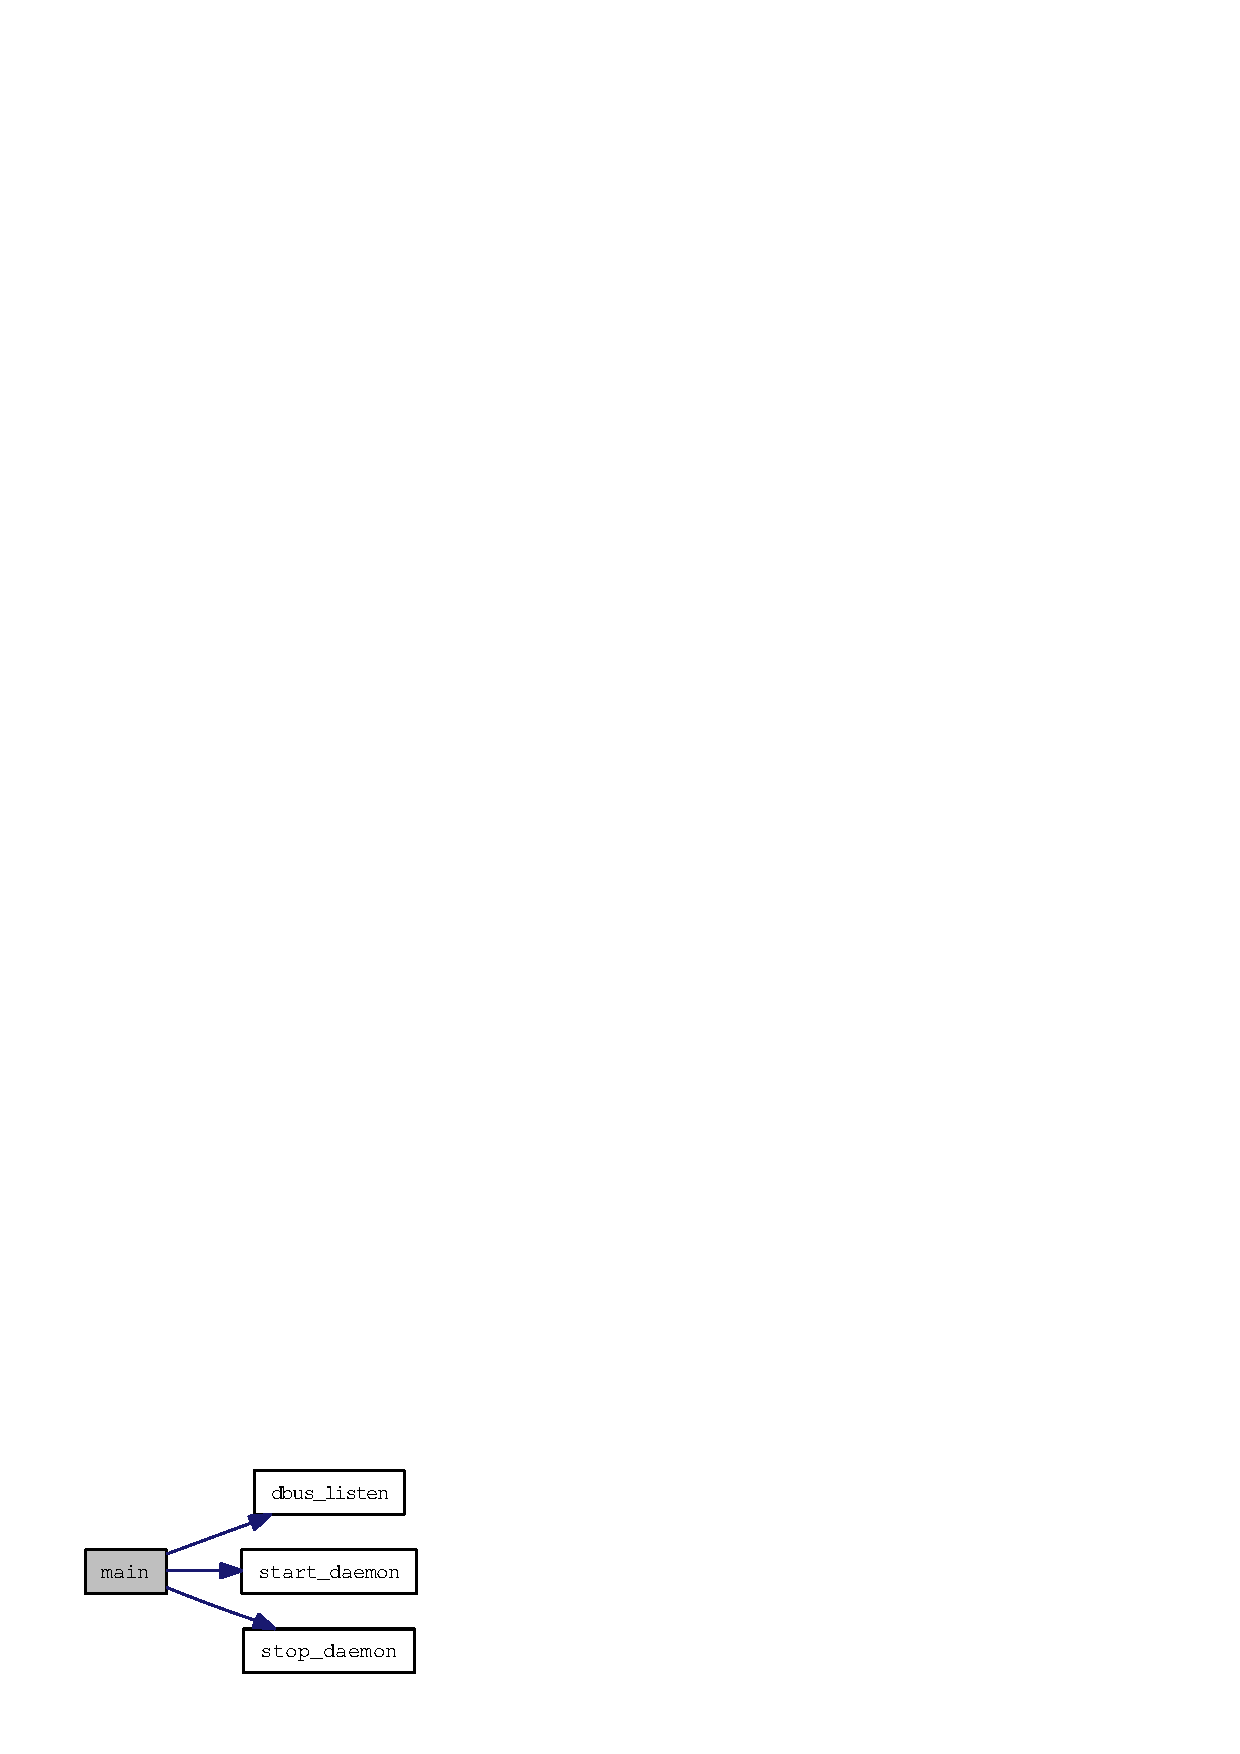
\includegraphics[width=102pt]{pf__daemon_8c_3c04138a5bfe5d72780bb7e82a18e627_cgraph}
\end{center}
\end{figure}
\hypertarget{pf__daemon_8c_0e2f72a981c64aefe314e745b28b6387}{
\index{pf\_\-daemon.c@{pf\_\-daemon.c}!start\_\-daemon@{start\_\-daemon}}
\index{start\_\-daemon@{start\_\-daemon}!pf_daemon.c@{pf\_\-daemon.c}}
\subsubsection{\setlength{\rightskip}{0pt plus 5cm}void start\_\-daemon ()}}
\label{pf__daemon_8c_0e2f72a981c64aefe314e745b28b6387}


Starts the program as a daemon and creates a lockfile (specified in the LOCKFILE constant). So it's impossible to start the daemon twice. 

Definition at line 45 of file pf\_\-daemon.c.

References LOCKFILE.

Referenced by main().

Here is the caller graph for this function:\nopagebreak
\begin{figure}[H]
\begin{center}
\leavevmode
\includegraphics[width=102pt]{pf__daemon_8c_0e2f72a981c64aefe314e745b28b6387_icgraph}
\end{center}
\end{figure}
\hypertarget{pf__daemon_8c_725630dc6f9856b1349100761924050f}{
\index{pf\_\-daemon.c@{pf\_\-daemon.c}!stop\_\-daemon@{stop\_\-daemon}}
\index{stop\_\-daemon@{stop\_\-daemon}!pf_daemon.c@{pf\_\-daemon.c}}
\subsubsection{\setlength{\rightskip}{0pt plus 5cm}void stop\_\-daemon ()}}
\label{pf__daemon_8c_725630dc6f9856b1349100761924050f}


Stops the daemon and deletes the lockfile, so a new instance can be started. 

Definition at line 69 of file pf\_\-daemon.c.

References LOCKFILE.

Referenced by main().

Here is the caller graph for this function:\nopagebreak
\begin{figure}[H]
\begin{center}
\leavevmode
\includegraphics[width=101pt]{pf__daemon_8c_725630dc6f9856b1349100761924050f_icgraph}
\end{center}
\end{figure}
